\subsubsection{Data Transfer}		
The following use cases pertain to how Condenser transfers data to the cloud. Figure~\ref{DataTransferUse} shows a diagram depicting the relationships between the data transfer use cases.
\begin{center}
	\begin{figure}[htbp]
		%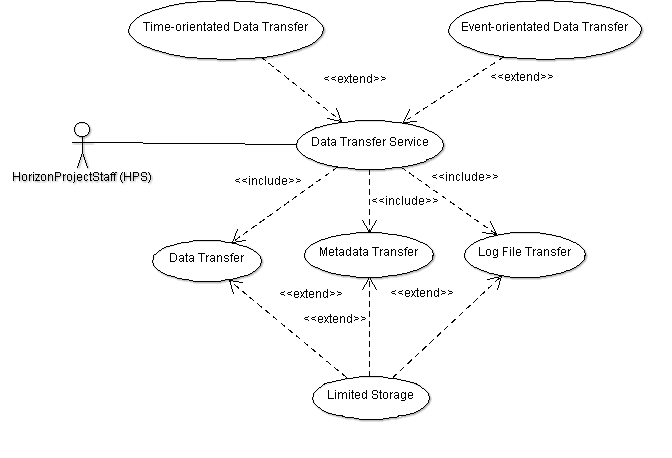
\includegraphics[scale=.5]{images/DataTransferUse.png}
		\caption{Use cases defining Condenser data transfer.\label{DataTransferUse}}
	\end{figure}
\end{center}	
\textbf{Use Cases:}\\
 
		\textbf{Data Transfer Service}\\	 
		\textbf{Participating Actors:} Horizon Partner (HP) and/or Project Participant(PP) \\
		\textbf{Event Flow:}
		\begin{enumerate}
\item The HP or PP initiates data transfer from one or more nodes to Condenser.
\item Data is cached locally.
\item When a data transfer event is initiated Condenser attempts to connect to and authenticate itself with one or more external data storage providers.
\item If there is external network connectivity then data is transferred off site (see time-orientated and event-orientated data transfer use cases) along with metadata see (see metadata transfer use case) and log information (see log file transfer use case). The data may be transferred periodically (see Time-orientated Data Transfer use case) or in response to events (see Event-orientated Data Transfer use case). 
\item See Handle unavailable connectivity use case for when connectivity to the external network cannot be established.
	    \end{enumerate}
		\textbf{Entry Conditions:} Condenser is setup and has a stable Internet connection.\\
		\textbf{Exit Conditions:} Data are transferred to external storage as well as cached locally.\\
		\textbf{Quality Requirements:} Bandwidth used for data transfer should be minimised.\\
		\line(1,0){350}	
 
		\textbf{Time-orientated Data Transfer}\\	 
		\textbf{Participating Actors:} Horizon Partner (HP) and/or Project Participant(PP) \\
		\textbf{Event Flow:}
		\begin{enumerate}
\item The HP or PP initiates data transfer from one or more nodes to Condenser.
\item Condenser attempts to connect to the external data storage system at fixed intervals or at particular points in time as given in the configuration rules -- see the set synchronization settings and set external storage connection settings use cases for more information.
\item If a connection is established, data, metadata and  log files are transferred to external storage. These will be encrypted if the configuration settings are set for this.
\item If a connection fails the non-transferred data are enqueued for subsequent transfer attempts.
	    \end{enumerate}
		\textbf{Entry Conditions:} Condenser is configured to do time-based synchronization and has a stable Internet connection.\\
		\textbf{Exit Conditions:} Data are transferred to external storage as well as cached locally.\\
		\line(1,0){350}		
		
		\textbf{Event-orientated Data Transfer}\\	  
		\textbf{Participating Actors:} Horizon Partner (HP) and/or Project Participant(PP) \\
		\textbf{Event Flow:}
		\begin{enumerate}
\item The HP or PP initiates data transfer from one or more nodes to Condenser.
\item Condenser attempts to connect to the external data storage system when particular events occur are per its configuration rules -- see the set synchronization settings and set external storage connection settings use cases for more information. For instance, an event could be that the local data cache has reached a particular size or that Internet bandwidth is at a particular threshold.
\item If a connection is established, data, metadata and  log files are transferred to external storage. These will be encrypted if the configuration settings are set for this.
\item If a connection fails the non-transferred data are enqueued for subsequent transfer attempts.
	    \end{enumerate}
		\textbf{Entry Conditions:} Condenser is configured to do event-based synchronization and has a stable Internet connection.\\
		\textbf{Exit Conditions:} Data are transferred to external storage as well as cached locally.\\
		\line(1,0){350}		
		
		\textbf{Metadata Transfer}\\	 
		\textbf{Participating Actors:} Horizon Partner (HP) and/or Project Participant(PP) \\
		\textbf{Event Flow:}
		\begin{enumerate}
\item The HP or PP initiates data transfer from one or more nodes to Condenser.
\item If there is external network connectivity then metadata is transferred off site. Condenser should deduplicate metadata and only transfer that which has not already been transferred. Duplication could otherwise arise because some metadata will pertain to many data points.
	    \end{enumerate}
		\textbf{Entry Conditions:} Condenser is setup and has a stable Internet connection.\\
		\textbf{Exit Conditions:} Metadata are transferred to external storage as well as cached locally.\\
		\textbf{Quality Requirements:} Bandwidth used for metadata transfer should be minimised.\\
		\line(1,0){350}	
		
\textbf{Log File Transfer} \\
		\textbf{Participating Actors:} Horizon Partner (HP) and/or Project Participant(PP) \\
		\textbf{Event Flow:}
		\begin{enumerate}
\item The HP or PP initiates data transfer from one or more nodes to Condenser.
\item If there is external network connectivity then log files are transferred off site. Condenser should use delta encoding to only transfer portions of log files that have not already been transferred.
	    \end{enumerate}
		\textbf{Entry Conditions:} Condenser is setup and has a stable Internet connection.\\
		\textbf{Exit Conditions:} Log files are transferred to external storage as well as cached locally.\\
		\textbf{Quality Requirements:} Bandwidth used for log file transfer should be minimised.\\
		\line(1,0){350}			
			 
		\textbf{Handling limited data storage} \\
		\textbf{Participating Actors:} Horizon Partner (HP) and/or Project Participant(PP) \\
		\textbf{Event Flow:}
		\begin{enumerate}
\item The HP or PP initiates data transfer from one or more nodes to Condenser.
\item If there is external network connectivity difficulties then its is possible that local data storage could fill up.
\item When the local data store is too full then Condenser should compress or aggregate or otherwise eliminate unnecessary data, metadata and log files as per Condenser's configuration settings (see Setup local database use case).
	    \end{enumerate}
		\textbf{Entry Conditions:} Condenser is configured with data handling rules.\\
		\textbf{Exit Conditions:} Data are compressed, aggregated or deleted to maximise space for new data.\\
		\line(1,0){350}	